\documentclass{beamer}
\usetheme{Warsaw}
\usecolortheme{seahorse}
\usepackage{amsmath}
\usepackage{amsfonts}
\usepackage{epstopdf}
\usepackage{amssymb}
\usepackage{graphicx}
\usepackage{movie15}
%\usepackage{CJKutf8}
\title{OpenLCDFDM: an finite-difference LCD simulator}
\author{\texorpdfstring{Zong-han, Xie\newline\url{icbm0926@gmail.com}}{Zong-han, Xie}}
\begin{document}
%\begin{CJK}{UTF8}{cwmc}
\begin{frame}
\titlepage
\end{frame}
\begin{frame}[label=licensepage]
\frametitle{License of this slide}
Introduction to Fourier transform and signal analysis by Zong-han, Xie (\href{icbm0926@gmail.com}{icbm0926@gmail.com}) is licensed under a Creative Commons Attribution-NonCommercial 4.0 International License. \newline
\begin{center}
\includegraphics[scale=1]{by-nc-sa.eps}
\end{center}
\end{frame}
\AtBeginSection[]
{
  \begin{frame}
    \frametitle{Outline}
    \tableofcontents[currentsection]
  \end{frame}
}
\begin{frame}
\frametitle{LCD on consumer products}
LCD on consumer products
\end{frame}
\begin{frame}
\frametitle{Principles of LCD display}
\end{frame}
\begin{frame}
\frametitle{Principles of LCD display}
\end{frame}
\begin{frame}
\frametitle{Principles of LCD display}
\end{frame}

\begin{frame}
\frametitle{References}
\begin{thebibliography}{0}
%\bibitem{SNGP} Supplementary Notes of General Physics by Jyhpyng Wang, \url{http://idv.sinica.edu.tw/jwang/SNGP/SNGP20090621.pdf}
\end{thebibliography}
\end{frame}

%---------------Examples of Latex---------
%\begin{frame}
%\frametitle{2nd page}
%\begin{block}{block}
%\begin{eqnarray}
%\frac{1}{2}
%\end{eqnarray}
%\end{block}
%\begin{alertblock}{alertblock}
%alertblock content
%\end{alertblock}
%\end{frame}
%\begin{frame}
%\frametitle{3rd page}
%\begin{itemize}
%\item<1-> 第一
%\item<1-> 2nd
%\item<2-> 3rd
%\item<3-> etc.
%\hyperlink{1stpage}{\beamerbutton{ooxx}}
%\end{itemize}
%\end{frame}
%\end{CJK}
\end{document}
